
\section{Introduction} \label{sec:introduction}
Todays programs are mostly highly configurable and customizable. Popular applications like Apache or MySQL can have a lot of configuration parameters as can be seen in \cref{fig:paramters}. With this large amount of  configuration options stake holders or customers can be satisfied easier since they can tailor a program to the their specific requirements. But with these big amount of options comes a bigger problem: \inlineQuote{unpredictability}. Looking at an example of Apache Storm (\cref{fig:ApacheStorm}) shows that the performance of two configurations of a program can differ significantly. \TODOX{figure einfügen} shows that solely changing a single parameter can increase the response time of Apache Storm by up to 100\%. Without using prediction methods such results are only visible after executing and measuring multiple, if not all, configurations of a system. Or in other words: when looking only at a single configuration, one cannot conclude whether that configuration is any good for the current requirements in.

\begin{figure}[h]
	\centering
	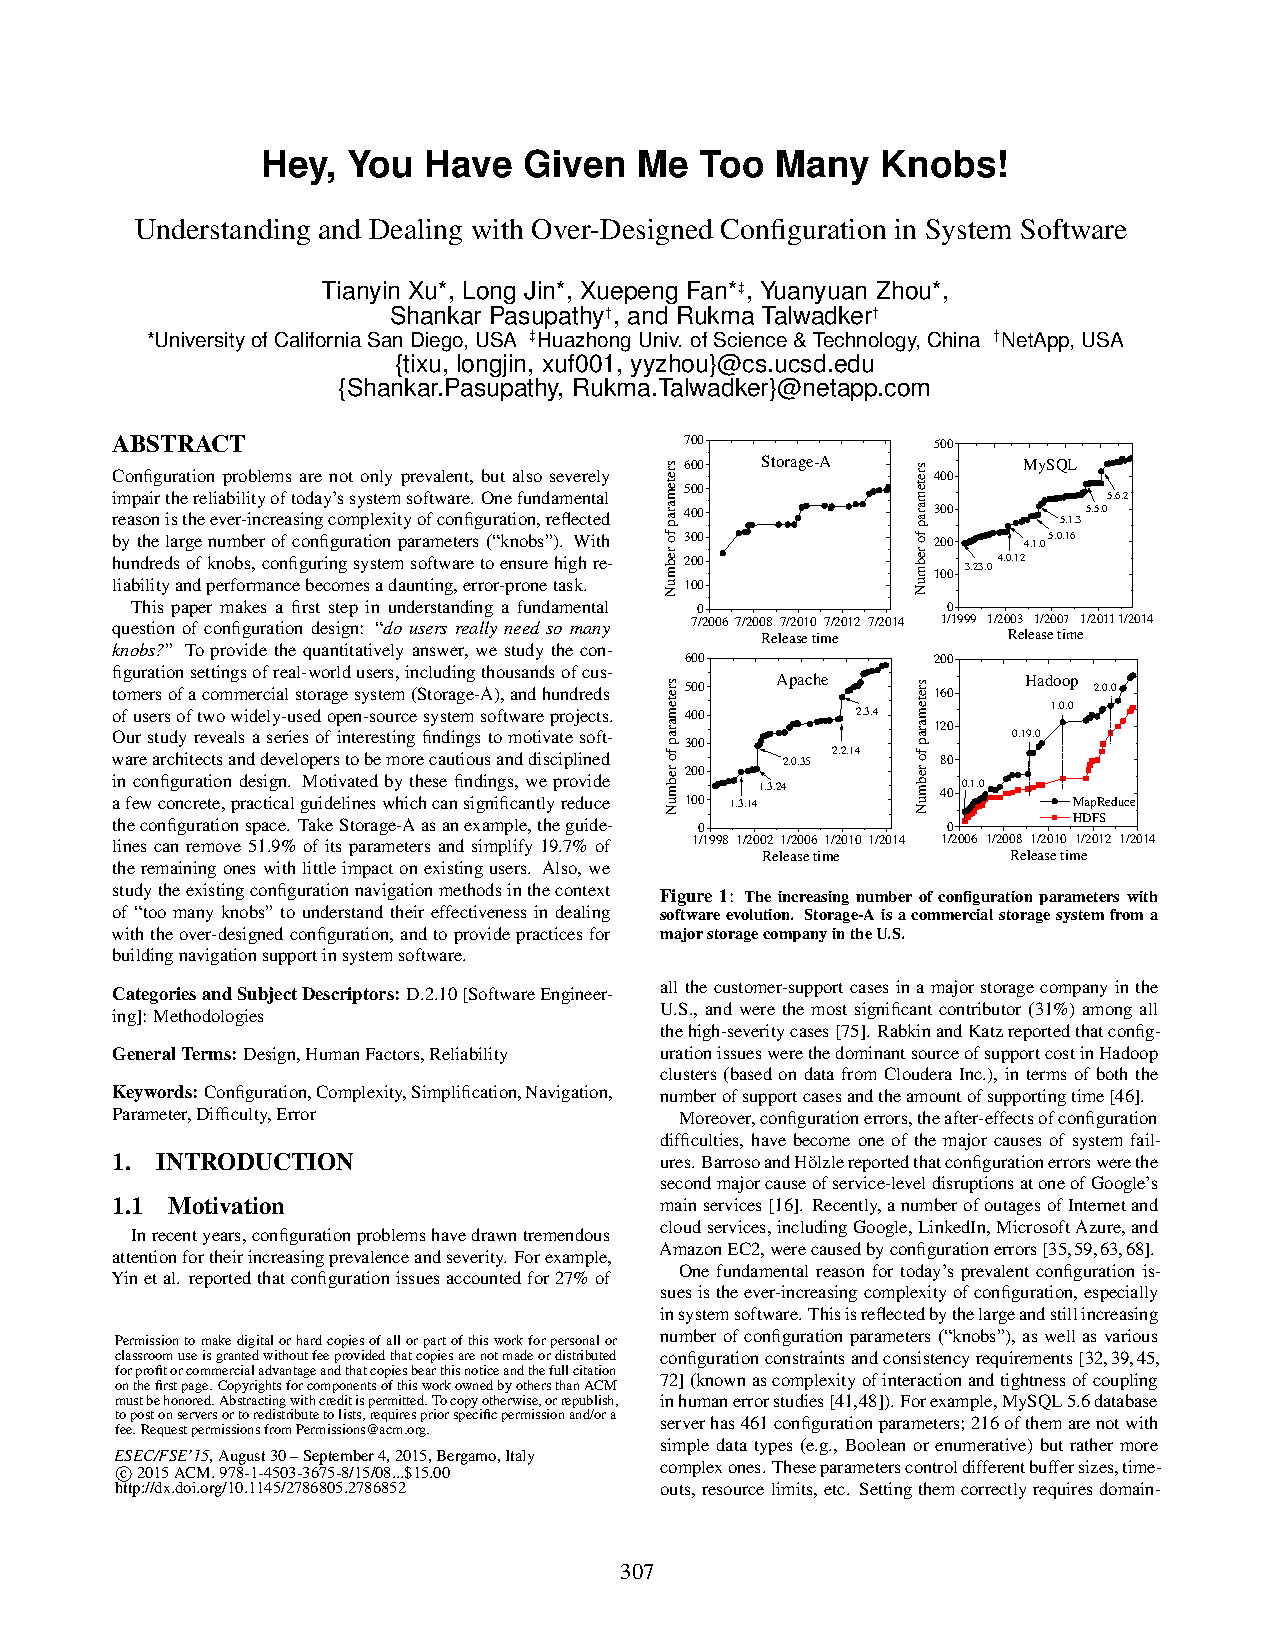
\includegraphics[clip,trim= 11cm 13cm 2cm 7cm]{Paper/thirdParty/HeyYouHaveGivenMeTooManyKnobs.pdf}
	\caption{Number of parameters of different popular programs \cite{YouveGivenMeTooManyKnobs}.}
	\label{fig:paramters}
\end{figure}\noindent
\begin{figure}[h]\noindent
	\begin{subfigure}{.45\linewidth}
		\centering
		\includegraphics[page=5,clip,trim=4cm 1cm 8cm 10cm,width=\linewidth]
		{Paper/thirdParty/vamos_keynote_norbert_siegmund.pdf}
		\caption{Configurations of Apache Storm sorted by measured throughput.}
	\end{subfigure}\hspace{.1\linewidth}
	\begin{subfigure}{.45\linewidth}
		\centering
		\includegraphics[page=5,clip,trim=17.4cm 1cm 0cm 10cm,width=.8\linewidth]
		{Paper/thirdParty/vamos_keynote_norbert_siegmund.pdf}
		\caption{Possible influences of only two options on the latency of Apache Storm. }
	\end{subfigure}
	\caption{Measurements done for Apache Strom that show an configurations can have a significant influence on the performance of a software system.}
	\label{fig:ApacheStorm}
\end{figure}


This is where prediction comes into play. By learning about the performance of some configurations of the system it tries to generates a function that can give an expected performance for a not measured configuration. This can be used to solve the just mention problem of finding a near optimal solution.
Further performance prediction can be used to find default configurations. These should be configurations that fulfills most requirements to an acceptable level. 
The most straight forward  approach to this problem would be a \textit{brute-force} solution. In this case that would mean measuring each and every single valid configuration. As we will see later in \TODOX{ref section} this approach is in general not feasible since the amount of valid configurations scales exponentially with the number of parameters. For that reason other approaches had to be found and especially the efficient sampling of a configuration space turned out to be a problem \cite{CostEfficientSampling_Gou_Siegmund_2015}. 

This paper will focus on showing different approaches and strategies to predicting the performance of a configurable software system. It will mainly discuss approaches developed by Norbert Siegmund et al. \cite{AutomatedFeatureDetectionSiegmund2012,VariabilityAwarePerformancePredictionJianmeiSigmundApel,CostEfficientSampling_Gou_Siegmund_2015, DistanceBasedSampling2019}. They will be explained and compared. More specificly this paper will have a look at 4 different approaches besides \textit{brute-force}.

The first discussed technique is \textit{Automated Feature Interaction Detection} (\AFID) \cite{AutomatedFeatureDetectionSiegmund2012}. The goal of this approach is to assign a performance influence value to each feature and feature interaction. This is done by observing and measuring the behavior of certain configurations. 
The other 4 approaches make use of a CART Tree as their learning choice but differ in the way they choose their sample. 
\textit{Variability Aware Performance Prediction} (\VAPP) \cite{VariabilityAwarePerformancePredictionJianmeiSigmundApel} uses random sampling to pick which configurations to compiled and measured. 
\WHAT~ \cite{DistanceBasedSampling2019}, as the next approach is called, tires a more mathematical way to find groups of similar configurations without actually measuring them. For this distance based clustering/sampling is used. 
The last two sampling approaches are proposed in the same paper by \citet{CostEfficientSampling_Gou_Siegmund_2015}. They \textit{Progressive} and \textit{Projective Sampling} are quite similar, since they both take advantage of the fact, that the general formular behind a learning curve is known. With this knowledge they generate a part of the actual curve and fit a function to it. Based on this function a optimal size for the actual sample set can be calculated. Both methods also take the cost of measurements and over-/underfitting into consideration.\\
All these approaches reach an accuracy of over 94\% on average in the conducted tests of their corresponding papers. This makes them good enough to be relevant for the topic of this paper.